\chapter{Adding Battery Awareness in EASY Backfilling}
\label{cha:heuristic}

\minitoc

After trying to introduce reinforcement learning in our model to choose the best compensation policy, this chapter describes a heuristic that englobes several elements to make better decisions. We named this heuristic \emph{\systemName}. This heuristic considers the power production and demand to find the best moment to compensate. Also, \emph{\systemName} mixes the compensations with the scheduling decisions. We present the algorithm, followed by the results compared with the previous heuristics.

\section{\systemName}

This heuristic acts in three different moments. First, Section \ref{sec:model_predictions} explains the predictions used through \emph{\systemName}'s decisions. These predictions are made at the beginning of the time window, just one time. Then, Section \ref{sec:model_easy} describes the modifications in the EASY Backfilling heuristic to introduce battery awareness. The modified EASY Backfilling acts every time a job finishes, arrives, or new servers are available. Finally, Section \ref{sec:model_compensations} defines the compensation policies. \emph{\systemName} compensates every time step.

\subsection{Predictions}
\label{sec:model_predictions}

As presented in Section \ref{sec:offline_plan}, ODM receives two predictions from offline modules: power production and power demand. Since ODM works online, it will not predict itself but use the predictions from offline. So, this section will not focus on the forecasting method but on using its results.

\begin{figure}[!htb]
    \centering
    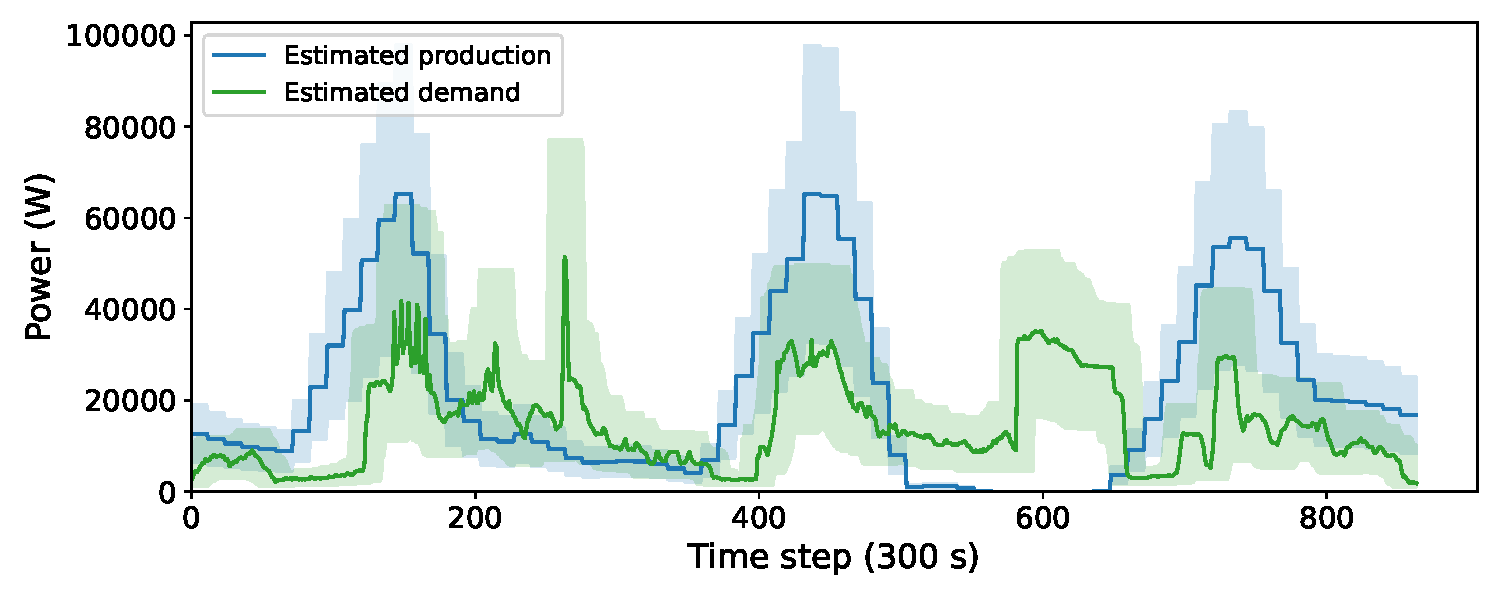
\includegraphics[scale=0.5]{Images/Heuristic/predictions.pdf}
    \caption{Renewable production and demand prediction. The blue (production) and green (demand) areas are the uncertainty given by the forecast.}
    \label{fig:predictions}
\end{figure}

Figure \ref{fig:predictions} illustrates both forecasts showing the area of uncertainty. The real value can be any value inside the uncertainty area. \emph{\systemName} uses these predictions to create different possible states of charge using equations \ref{equ:battery_energy} and \ref{equ:battery_state_of_charge}. To do so, we estimated $P_{dch}$ and $P_{ch}$ using Equations \ref{equ:battery_charge}, and \ref{equ:battery_discharge}: 
\begin{equation}
    \label{equ:battery_charge}
    P_{ch}(t) = 
    \begin{cases}
        P_{renew}^{est} - P_{load}^{est},& \text{if } P_{renew}^{est} > P_{load}^{est} \\
        0,              & \text{otherwise}
    \end{cases}
\end{equation}
\begin{equation}
    \label{equ:battery_discharge}
    P_{dch}(t) = 
    \begin{cases}
        P_{load}^{est} - P_{renew}^{est},& \text{if } P_{renew}^{est} < P_{load}^{est} \\
        0,              & \text{otherwise}
    \end{cases}
\end{equation}

Where:
\begin{itemize}
    \item \(P_{renew}^{est}\): Estimated power production from renewable;
    \item \(P_{load}^{est}\): Estimated power demanded.
\end{itemize}

\begin{figure}[!htb]
    \centering
    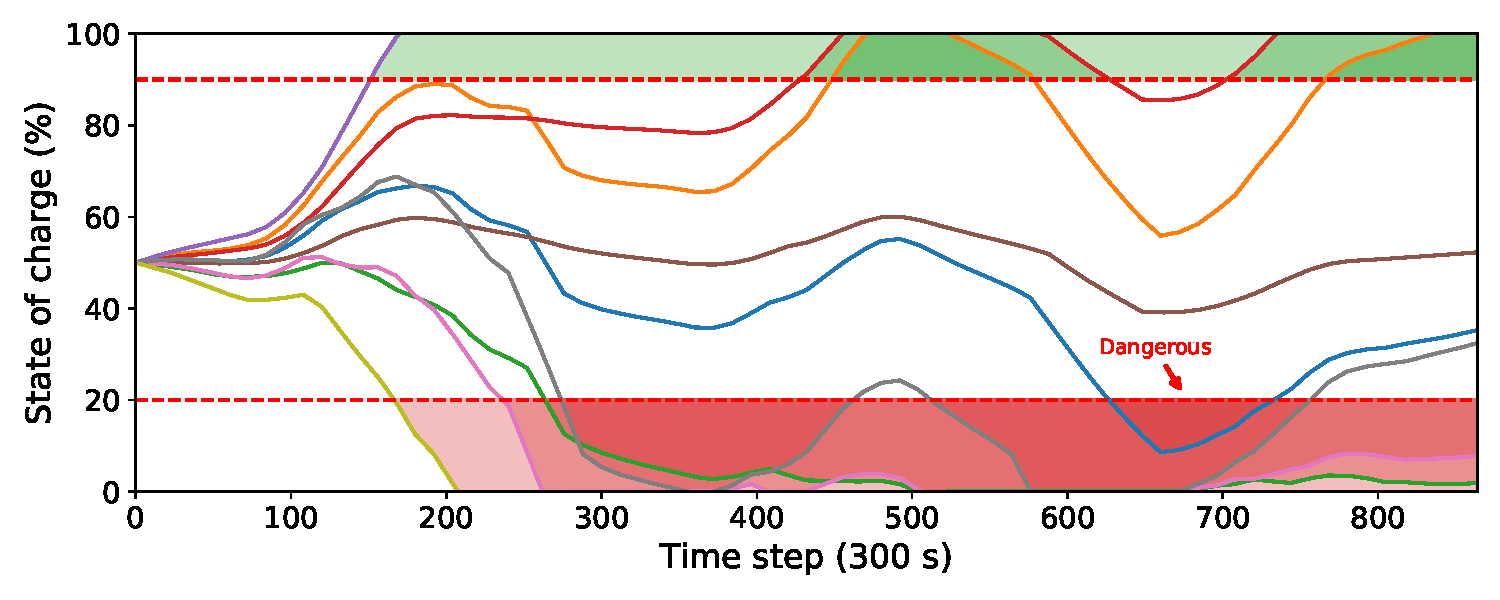
\includegraphics[scale=0.5]{Images/Heuristic/state_of_charge.pdf}
    \caption{Result of the Equation \ref{equ:battery_state_of_charge} for different predictions. The dangerous area is when 5 or more curves (so, more than half of them) are below 20\%.}
    \label{fig:estimated_state_of_charge}
\end{figure}

Figure \ref{fig:estimated_state_of_charge} demonstrates the result of applying Equation \ref{equ:battery_state_of_charge} using nine different predictions. \emph{\systemName} calculates these SoC combining lower, median, and upper boundaries from the area presented in Figure \ref{fig:predictions} (e.g., demand lower boundary + production lower boundary, demand median + production lower boundary, demand median + production higher boundary, etc...). It is possible to notice that the state of charge can vary a lot. Section \ref{sec:model_compensations} will describe how we use these SoCs to compensate. Figure \ref{fig:estimated_state_of_charge} also illustrates both SoC upper and lower thresholds (red dashed lines). Setting upper and lower thresholds helps to increase the battery lifetime \cite{xu2016modeling}. The narrower the range, the longer the expected lifetime \cite{xu2016modeling}. However, selecting a narrow range limits the battery benefits. The figure presents both thresholds as 90-20\%, but they are parameterizable. Finally, \emph{\systemName} estimates dangerous areas in the time window. Figure \ref{fig:estimated_state_of_charge} indicates this moment. It considers the dangerous areas when more than half of the predicted SoC curves are below the lower threshold. Taking Figure \ref{fig:estimated_state_of_charge} example with nine predictions, \emph{\systemName} considers the dangerous point where five curves are below 20\%. Section \ref{sec:model_easy} will explain how it uses these moments to make better scheduling decisions.


\subsection{Job Scheduling}
\label{sec:model_easy}

One of the most important ODM's duties is placing jobs on servers. To do so, \emph{\systemName} implements EASY backfilling using two different sorts \cite{mu2001utilization, lelong2018tuning}. We detail how we use both sorts in this section. Algorithm \ref{alg:algo_scheduling_heuristic} presents the main idea. This algorithm is similar to Algorithm \ref{alg:algo_scheduling} but with some modifications (we highlighted them). \emph{\systemName} runs this algorithm when a job arrives, finishes, or new servers are available. First, this heuristic sorts the jobs in the queue in a priority order $P_{R}$ (line 2). Then, it finds the servers to run this job (line 5). The server must be available at least at the actual time step to be chosen. Line 6 has the first modification. Usually, EASY backfilling only verifies if the server's $S$ is available now. We added the following verifications:

\begin{enumerate}
    \item It verifies if the server's $S$ is available during the entire execution, considering the walltime given by the user as the execution time. If so, it returns true. If not, it goes to the next verification;
    \item It verifies if it is possible to change the plan to keep the servers S running the entire execution. To do so, it does the following steps:
    \begin{enumerate}
        \item First, it calculates how much energy is needed. Let's say $Ed_t$ is the energy demanded in step $t$ without modification and $Ed_t^{'}$ is with modification. So, it calculates $Ed_t^{'}$ for each time step $t$ that the server sleeps, putting the server in the same state/speed as the previous time step ($t-1$). The total energy demanded is $\sum Ed_t^{'} - Ed_t$ considering all the time steps that the job executes;
        \item Then, it calculates how much energy is possible to take from future steps, putting idle servers to sleep. Let it be $E_{poss}$. Since we need to maintain the state of charge between both thresholds, we can not "migrate" all the energy to use now. So, it only considers the idle servers from the actual time step until the time step where the SoC will be equal or lower to the lower threshold. We can migrate the energy freely between the actual time step and this future one. Figure \ref{fig:idle_machines_verification} illustrates this verification;
        \item Then, it tests if $E_{poss} >= \sum Ed_t^{'} - Ed_t$. If this is false, it returns false and does not change the plan. If this is true, it makes $Ed_t = Ed_t^{'}$, changes the server speeds, and recalculates the planned state of charge (using Equation \ref{equ:battery_state_of_charge}).
    \end{enumerate}
\end{enumerate}

\IncMargin{1em}
\begin{algorithm}[!htb]
    \LinesNumbered
    \footnotesize
    \SetAlgoLined
    \SetKwInOut{Input}{input}\SetKwInOut{Output}{output}
    \Input{Queue $Q$ of waiting jobs, $P_{R}$ as priority order, and $P_{B}$ as backfilling order.}
    \Output{None (calls to \textit{Start()})}
    \Begin{
        Sort $Q$ according to $P_{R}$\;
        \For{job $j$ in $Q$}{
            Pop $j$ from $Q$\;
            $S \leftarrow$ \textit{select\_servers($j$)}\;
            \uIf{\hl{$j$ can be started and finished in servers $S$}}{
                \textit{Start($j$, $S$)}\;
            }\Else{
                Reserve $j$ at the earliest time possible according to the walltime of the currently running jobs\;
                Sort $Q$ according to $P_{B}$\;
                \For{job $j^{'}$ in $Q$}{
                    $S \leftarrow$ \textit{select\_servers($j^{'}$)}\;
                    \If{\hl{$j^{'}$ can be started and finished in servers $S$ without delaying the reservation on $j$}}{
                        \textit{Start($j^{'}$, $S$)}\;
                    }
                }
                \textbf{break}\;
            }
        }
    }
    \caption{\emph{\systemName} scheduling. Modified from \cite{lelong2018tuning}.}
    \label{alg:algo_scheduling_heuristic}
\end{algorithm}
\DecMargin{1em}

\begin{figure}[!htb]
    \centering
    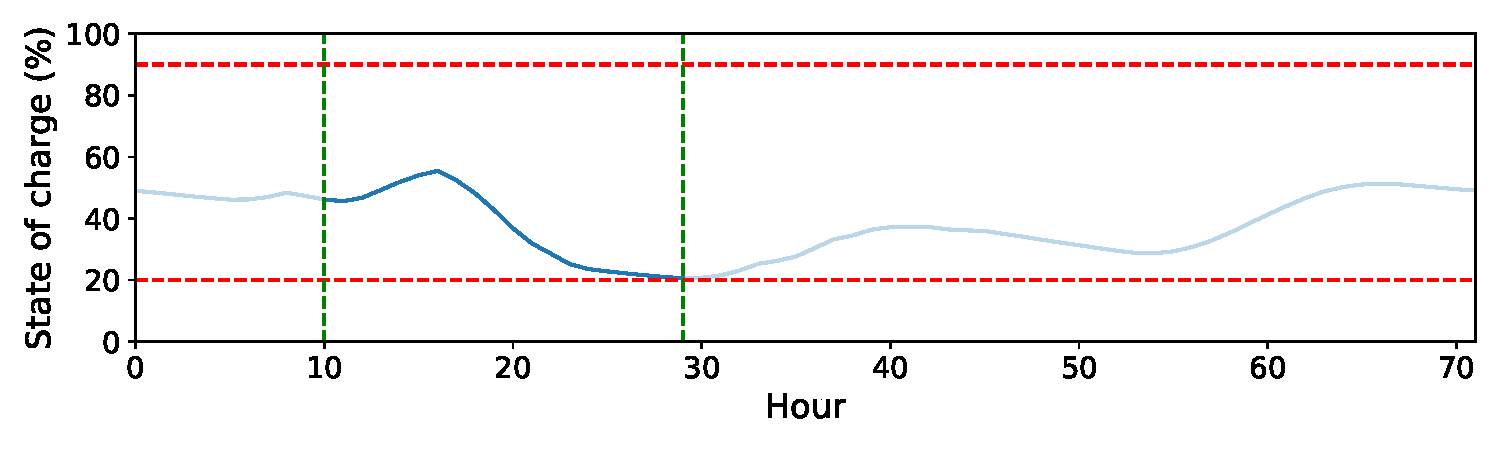
\includegraphics[scale=0.5]{Images/Heuristic/idle_machines.pdf}
    \caption{Verification of possible energy to save. In this example, the actual step is at hour 10. In this step, it needs to verify how much energy is possible to save from future steps. So, it verifies the idle servers from hour 10 to hour 29, because at hour 30 the state of charge is equal to 20\%. It can change the usage from hour 10 to hour 29 freely. Taking energy from after hour 30 could violate the lower threshold since we will use more energy from the batteries.}
    \label{fig:idle_machines_verification}
\end{figure}

These verifications do not increase the complexity. Verification 1 goes through the plan with limited size (e.g., in our three-day time window, we have a plan with 864 time steps). Verification 2-a is done together with verification 1. Verification 2-b is faster than the others since it can process fewer steps and stop when $E_{poss} >= \sum Ed_t^{'} - Ed_t$. Verification 3-c is just to apply the modifications. It recalculates the state of charge to maintain the SoC updated for the next jobs to schedule. So, if a job puts a future state of charge close to the lower threshold, the next job takes it into account. Continuing in algorithm \ref{alg:algo_scheduling_heuristic}, if the tests pass, then it starts the job (line 7). When it finds a job that can not be placed now, the algorithm does the backfill process (lines 9-17). Then, it finds the first moment to run this job (named priority job) in the future (line 9). So, it re-sorts the queue using $P_{B}$ (line 10), placing the other jobs in the servers (lines 11-16) without delaying the (future) priority job execution (line 13). Line 13 does the same verification as line 6.

As mentioned before, EASY backfilling sorts the jobs by $P_{R}$ and $P_{B}$. Our implementation starts with $P_{R}$ using Bounded Slowdown from Equation \ref{equ:slowdown}. Bounded Slowdown estimates the ratio between the total time a job stays in the system and its actual processing time. This order helps to let a job wait proportionately to its size. For $P_{B}$, \emph{\systemName} sorts the waiting queue by the smallest sizes first (walltime multiplied by the number of resources needed). This order helps in the backfill process since sometimes the "holes" in the scheduling demand very small jobs. Also, these jobs are less likely to demand more energy from future time steps (\emph{\systemName} lets the energy to the priority ones). Figure \ref{fig:estimated_state_of_charge} highlights a dangerous area. In this area, \emph{\systemName} changes $P_{R}$ to also use the smallest sizes first. These are not good moments to start big jobs, even if they are waiting too long in the queue. Small jobs demand less energy and are more likely to finish.

\subsection{Power compensation}
\label{sec:model_compensations}

After describing the scheduling algorithm, this section explains the heuristic to compensate for power fluctuations. While the scheduling algorithm runs for every job arrival, end, or server state modification, the power compensation algorithm will execute at every new time step. Since the scheduling algorithm modifies future time steps (it places the jobs in servers that are already on) and verifies the violations, we do not need to run the power compensations for every placement. Also, changing the server state too much between on and off can degrade it faster and takes time to power on/off. So, we defined that the state and speed stay constant inside each time step. 

The main objective of this part of the heuristic is to finish the time window with the state of charge as close as possible to the planned. Renewable sources can produce more or less than predicted. Also, the power usage can vary due to server idleness or scheduling modifications. So, at each time step, \emph{\systemName} calculates the state of charge for all future time steps using Equation \ref{equ:battery_state_of_charge}. Then, it calculates the energy difference $E_{comp}$ between the target and the estimated SoC at the end of the time window using Equations \ref{equ:delta_energy} and \ref{equ:energy_battery}. \emph{\systemName} needs to reintroduce/remove the energy $E_{comp}$ before the end of the time window.

When the compensation is positive ($E_{comp}>0$), we can increase the speed of the servers or run more jobs. First, \emph{\systemName} uses the $E_{comp}$ to speed up the running jobs. It goes improving from the actual step until the last step. In each step, \emph{\systemName} increases the processor's speed of the running jobs on this step. So, it tends to put more energy into the jobs right now than in the future. This behavior helps in avoiding jobs to reach their walltime. After that, if there is still energy, it verifies if there are jobs in the waiting queue. If so, it turns on some servers to run these jobs. If there is not or it turned all the servers needed to run jobs, it lets the remaining energy in the battery. This is a conservative approach. \emph{\systemName} could be aggressive, using the remaining energy to turn on machines in the future. However, we prefer to finish with more energy in the batteries than expend this energy not wisely.

In the negative compensation ($E_{comp}<0$), \emph{\systemName} considers the estimated SoCs from Figure \ref{fig:estimated_state_of_charge}. First, it finds the time step with the higher number of predictions below 20\% or the last time step if there are no predictions below 20\% (let's name it the violation time step). The idea is to reduce the usage before the violation, reducing the violation probability. Then, \emph{\systemName} reduces servers speed in the following order (stopping when it is enough):
\begin{enumerate}
    \item Impacts idle servers from the violation time step to the actual time step (it goes through the time steps backward);
    \item Impacts idle servers from the violation time step to the last time step (it goes through the time steps forward);
    \item Impacts running servers from the violation time step to the last time step (it goes through the time steps forward);
    \item Impacts running servers from the violation time step to the actual time step (it goes through the time steps backward);
\end{enumerate}

\emph{\systemName} focuses first on idle servers because impacting running servers can increase the number of killed jobs. Killing jobs increases wasted energy. So, \emph{\systemName} searches for idle servers in both ways (violation time step $\rightarrow$ actual time step and violation time step $\rightarrow$ last time step). If reducing the usage from idle servers is insufficient, we start to impact running servers (steps 3 and 4). Our idea is to impact them as far as possible from the actual step, considering the violation step. The real total job execution time is uncertain (e.g., they could finish earlier than predicted). If we change the order (step 4 before step 3), the chance of really impacting the job is higher since it will reduce the energy from the violation step to the actual step. Doing step 3 before, we expect that the job finishes before these changes, while impacting the steps around the violation step. 

\section{Results Evaluation}

After presenting \emph{\systemName}, we compare its results with the algorithms presented previously. We execute the same critical cases and 100 average cases presented in Section \ref{sec:experiment_environment}. Just to remember, the critical cases are:
\begin{enumerate}
    \item \emph{Critical 1}: Profile best-case and workload in the beginning;
    \item \emph{Critical 2}: Profile best-case and workload in the end;
    \item \emph{Critical 3}: Profile worst-case and workload in the beginning;
    \item \emph{Critical 4}: Profile worst-case and workload in the end;
\end{enumerate}

The average cases are the 100 workloads and power productions generated by Gaussian noise over 10 different traces of each (workload and power production). The results of the baselines and policies are the same as the previous sections.

\subsection{Critical cases}

\subsubsection{Scenario Critical 1}

Figure \ref{fig:beasy_critical_1} illustrates all the results obtained for the execution with the profile best-case and workload in the beginning. This scenario has more space for improvement because the job majority arrives on the first day, and we have more energy to finish them than predicted. So, the heuristics have time to decide when to start the jobs and how to approximate the target SoC. The best algorithm is \emph{\systemName}, with 99.01\% finished jobs in number and 96.07\% size. Also, the jobs not finished are postponed and not killed. It ends above the target SoC. Regarding wasted energy, it is possible to notice that \emph{\systemName} better expends the energy received, resulting in a saving of 35.33\% compared with the second-best wasted energy result (\emph{Workload reactive}). It has a higher bounded slowdown compared to the policies but a lower mean than the baselines. It runs more jobs, which makes more jobs wait longer. However, it maintains all slowdowns below 100, while all other algorithms have some jobs with higher slowdowns.

\begin{figure}[!htb]
    \centering
    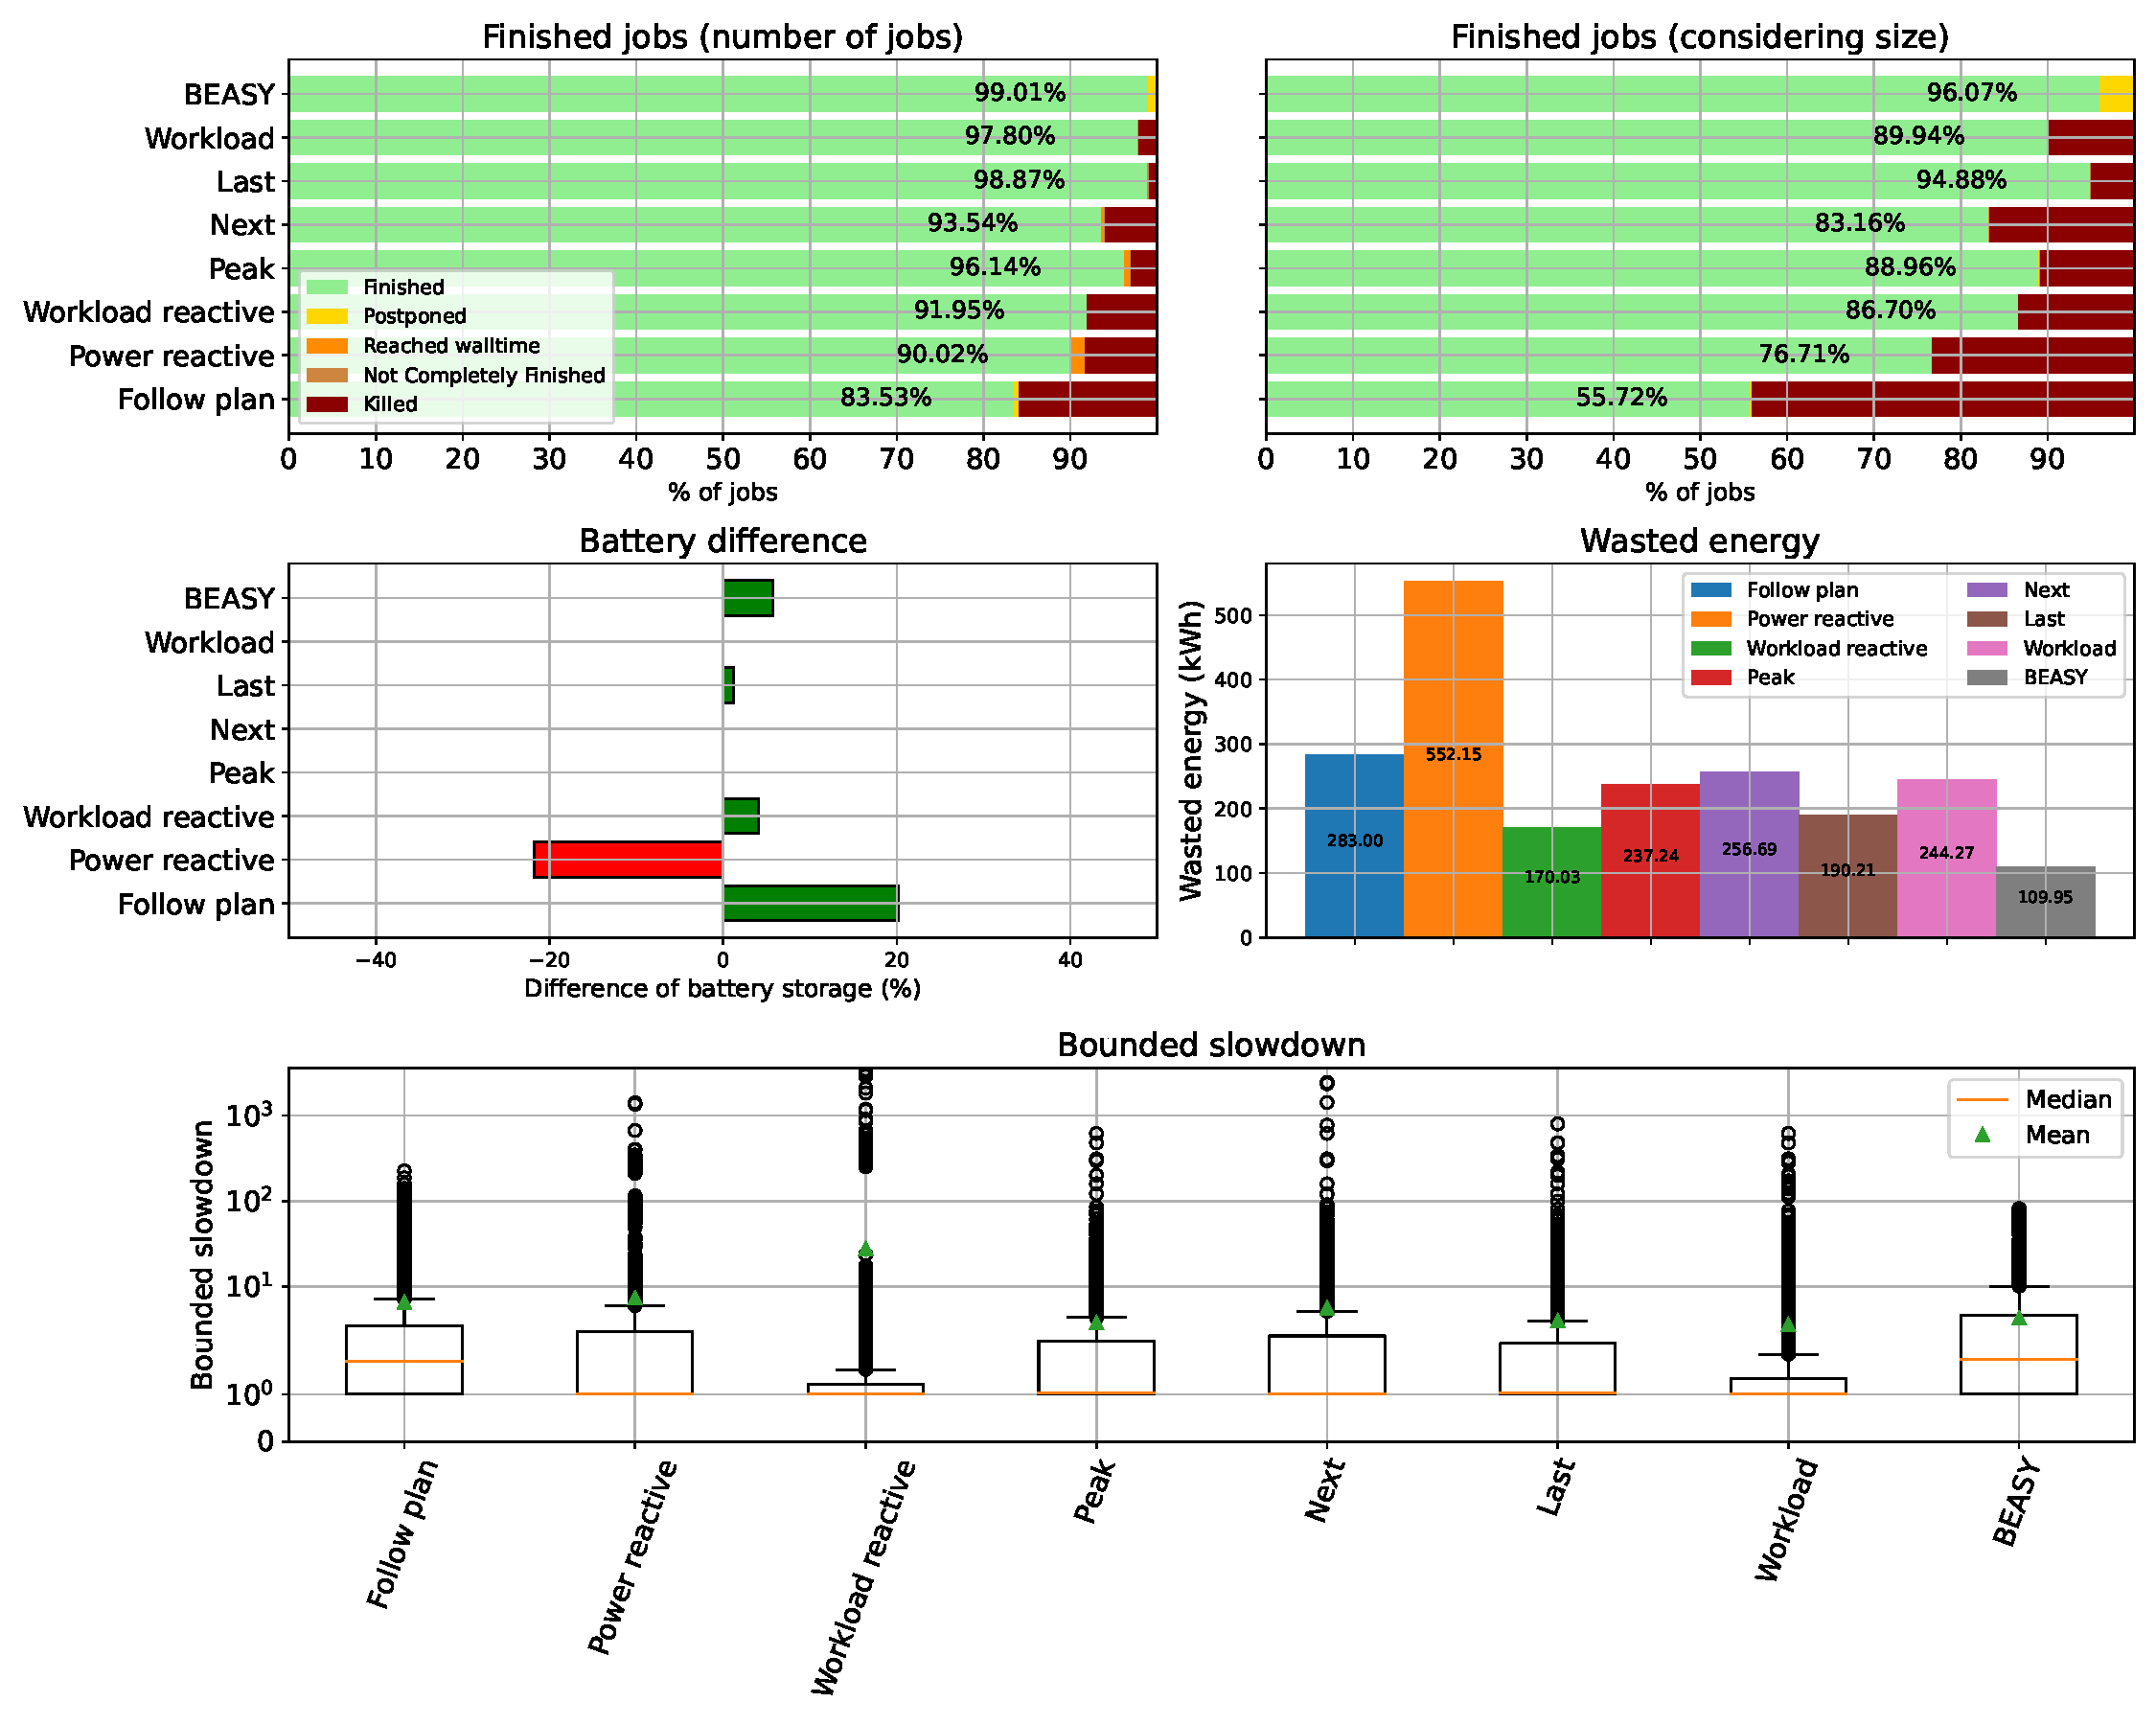
\includegraphics[scale=0.39]{Images/Heuristic/profile_best_workload_1_with_noise.pdf}
    \caption{Results of \emph{\systemName} on critical case 1.}
    \label{fig:beasy_critical_1}
\end{figure}

\emph{Workload reactive} execution kills 8.05\% of jobs. This heuristic is too aggressive compared to \emph{\systemName}. As mentioned before, \emph{Workload reactive} puts all jobs to start as soon they arrive. So, it dries the battery too fast. Figure \ref{fig:critical_soc_s1} compares the state of charge of the \emph{Workload reactive} and \emph{\systemName}. \emph{Workload reactive} dries too fast the battery and needs to kill the jobs, while \emph{\systemName} is conservative. We can see in this scenario that \emph{\systemName} makes better decisions than all other executions. Here, being conservative helped in the result. It finishes more than 99\% of the submitted jobs, guaranteeing they have the energy to finish. The 1\% is postponed to the next time window. We discuss this approach later. Also, it finishes saving energy in the battery, which can help the next time step to run the postponed jobs.

\begin{figure}[!htb]
    \centering
    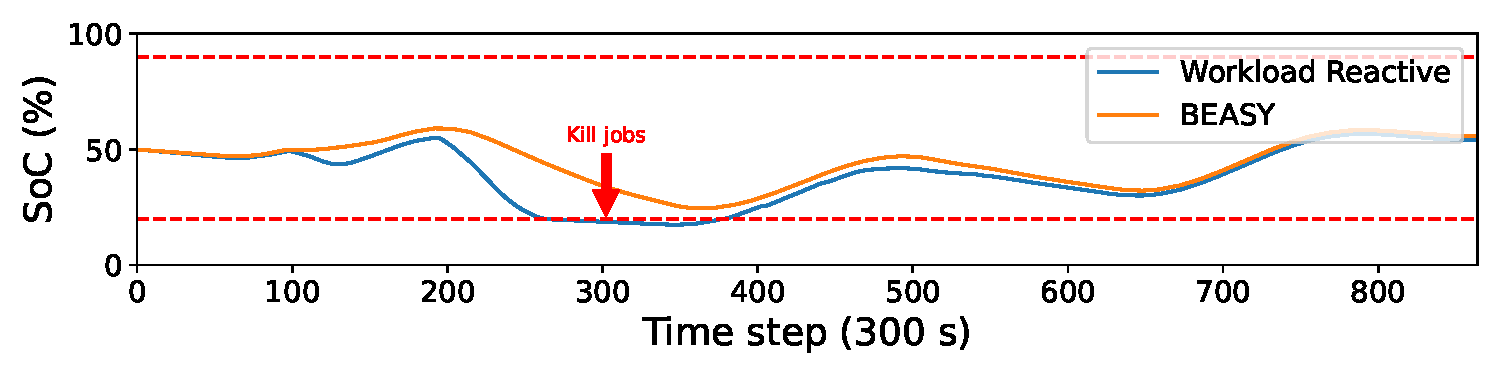
\includegraphics[scale=0.5]{Images/Heuristic/critical_soc_s1.pdf}
    \caption{Comparison between the state of charge of \emph{Workload reactive} and \emph{\systemName}.}
    \label{fig:critical_soc_s1}
\end{figure}

\clearpage

\subsubsection{Scenario Critical 2}

The second case is more complicated than the previous one. Here, the job majority arrives on the last day of the time window. So, the algorithms have a shorter time to schedule them. Figure \ref{fig:beasy_critical_2} illustrates the results. \emph{\systemName} is the second best in finished jobs in number. Considering the size, it has lower finished jobs than \emph{Workload} and \emph{Last} policies. However, \emph{\systemName} does not kill any job, while \emph{Workload} and \emph{Last} policies kill almost 5\% (in number). Only \emph{Workload reactive} is better than \emph{\systemName} in finished and killed jobs (in number and size). As mentioned before, this is the perfect scenario for the \emph{Workload reactive} approach. Considering the battery level, \emph{\systemName} ended with more energy in the battery. Since the jobs arrive at the end of the time window, \emph{\systemName} prefers to save this energy than starting jobs without knowing if they would finish. \emph{Workload reactive} starts the jobs, ignoring the target level and resulting in a deficit of energy in the battery. Considering the wasted energy, \emph{\systemName} wasted 22.10\% more energy than \emph{Workload reactive}, but it wasted less than all the other algorithms. Finally, \emph{\systemName} has a similar bounded slowdown to \emph{Workload reactive}, but with some values above 100. Again, it is complicated to compare algorithms with different jobs finished. But it has a better slowdown than the other algorithms.
 
\begin{figure}[!htb]
    \centering
    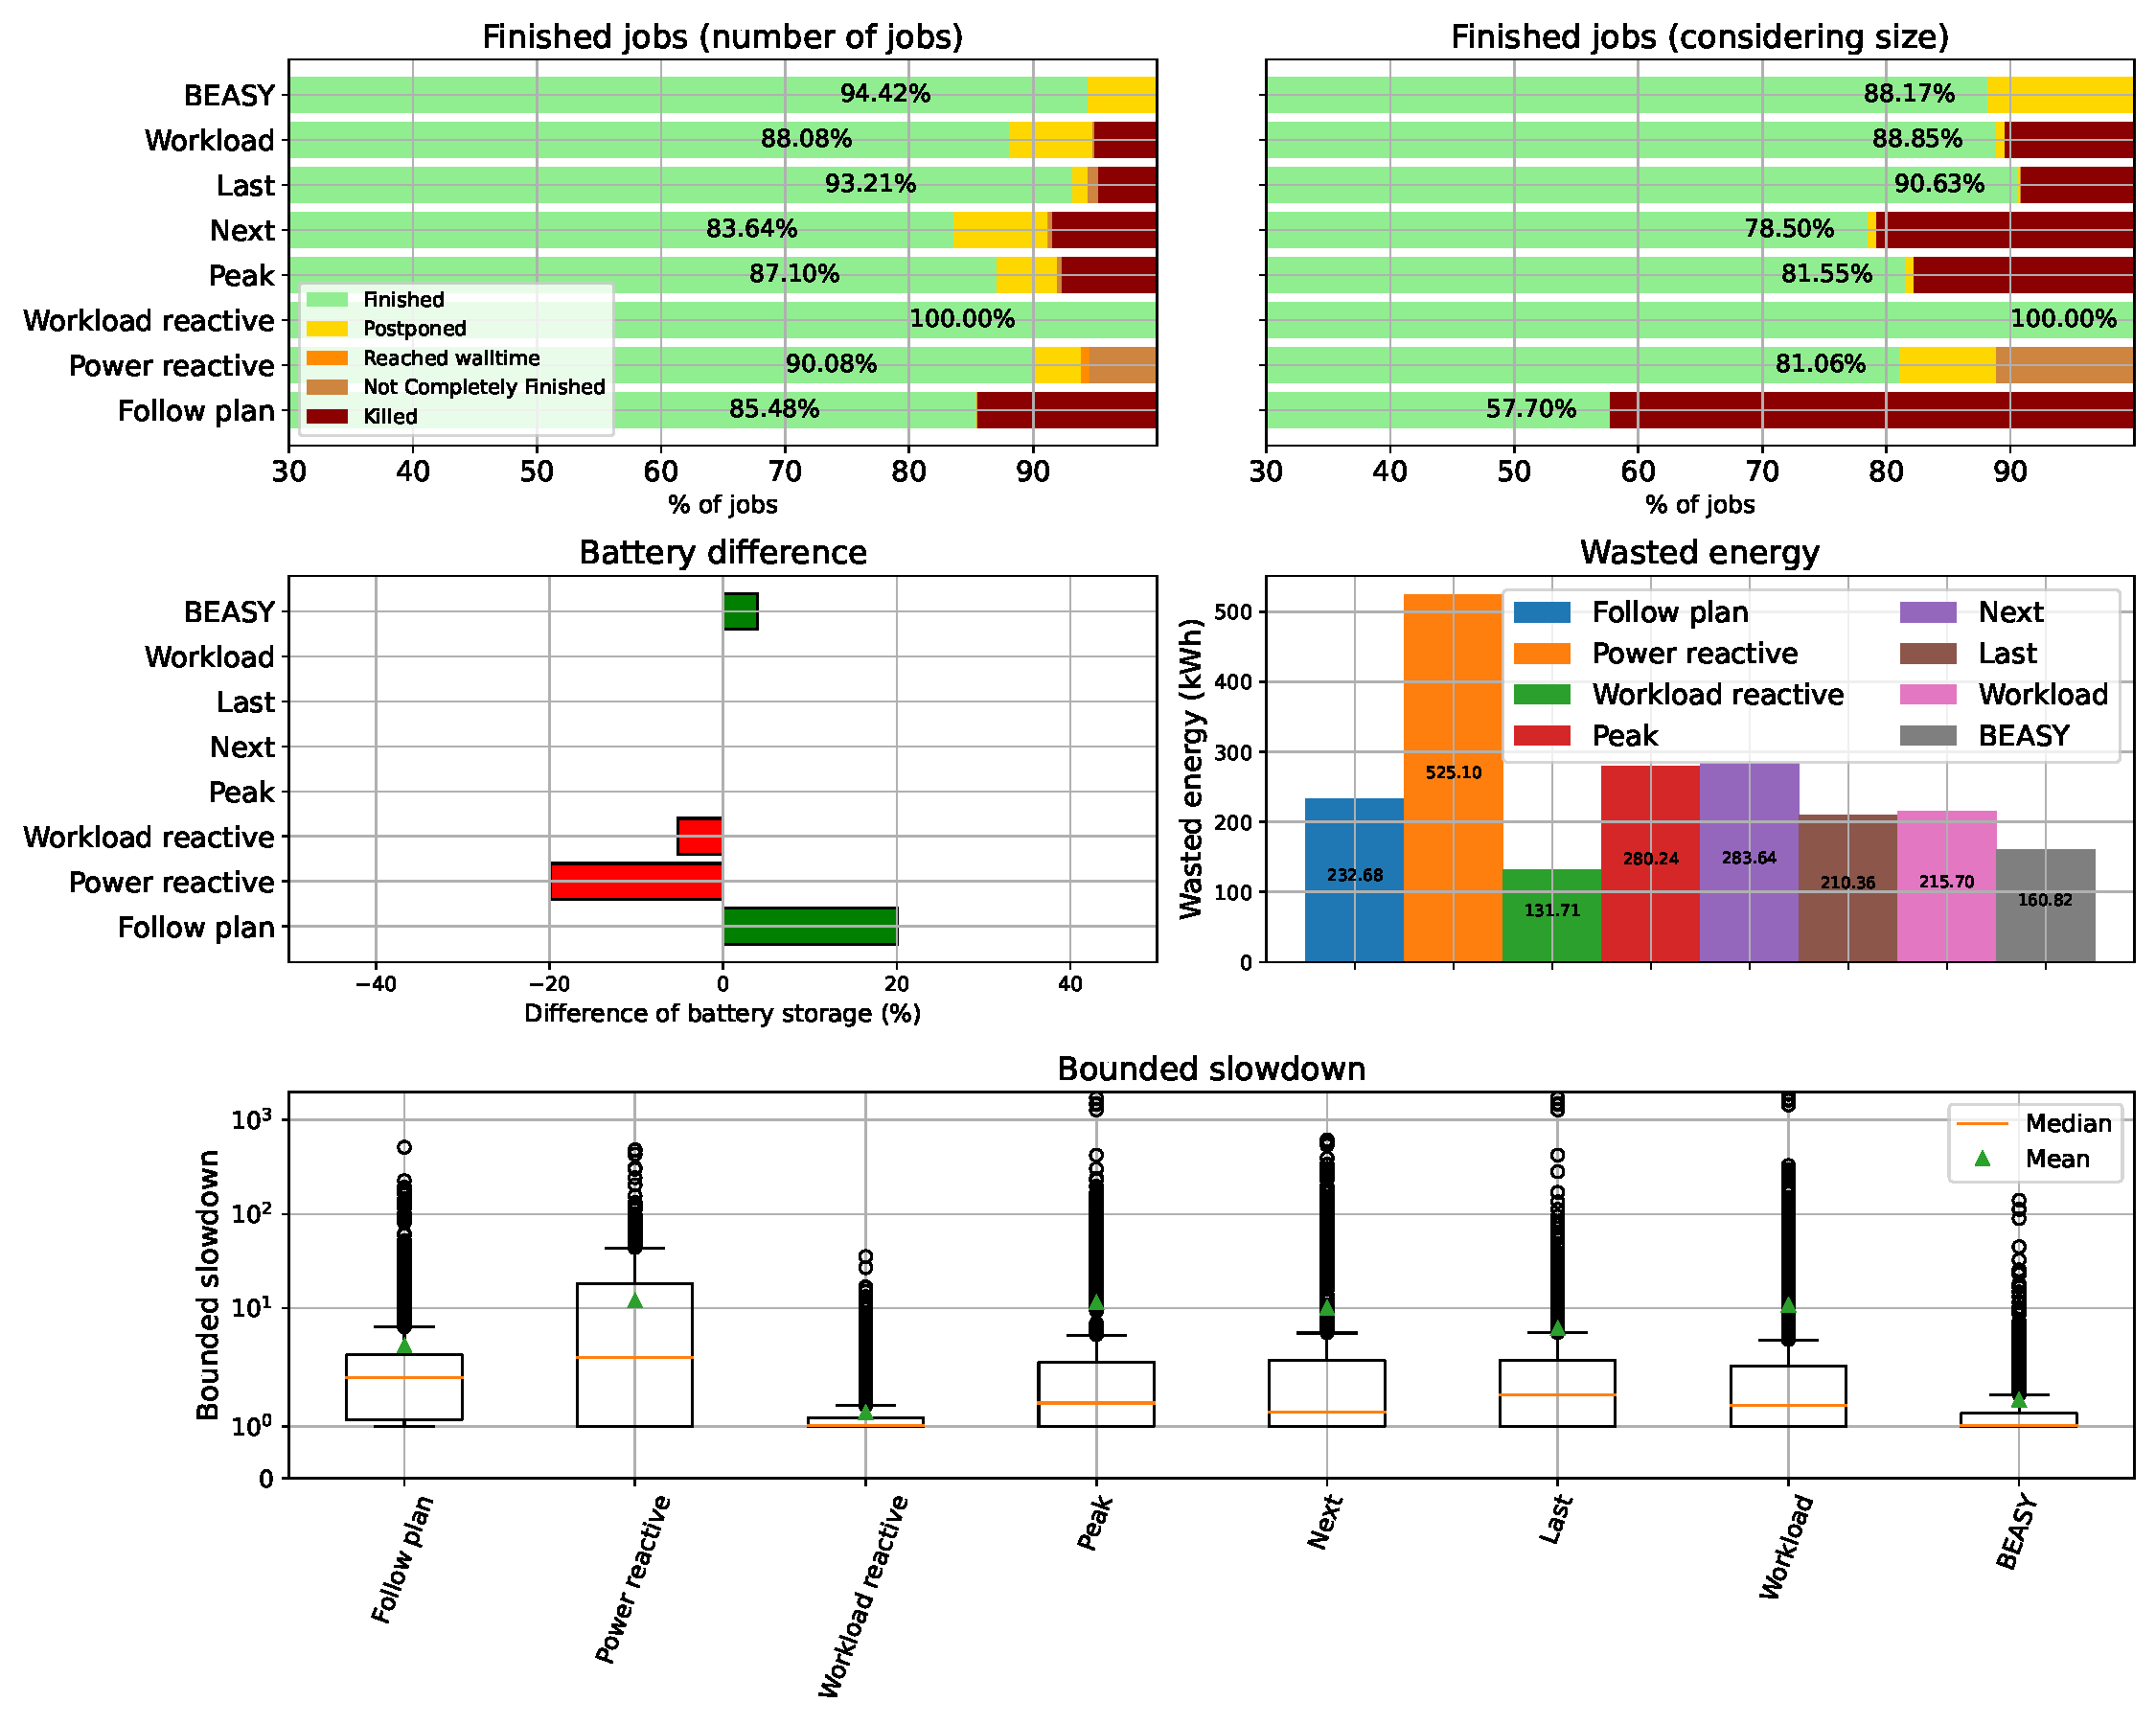
\includegraphics[scale=0.39]{Images/Heuristic/profile_best_workload_2_with_noise.pdf}
    \caption{Results of \emph{\systemName} on critical case 2.}
    \label{fig:beasy_critical_2}
\end{figure}

\clearpage

\subsubsection{Scenario Critical 3}

The third case is with the worst-case profile and workload in the beginning. In this case, the algorithms have time to schedule the jobs but receive way less energy coming from renewable. So, besides finding the best moment to place the jobs, they must adapt their power usage. Figure \ref{fig:beasy_critical_3} demonstrates the results. \emph{\systemName} is the second best in finished jobs, very close to the best one \emph{Power reactive}. Also, \emph{\systemName} kills very few jobs (0.10\%). Considering the size, \emph{\systemName} is the best one, finishing more than the \emph{Power reactive}. Comparing \emph{\systemName} and \emph{Power reactive}, the former has a better battery level. \emph{Power reactive} finishes with more than 20\% of battery deficit. \emph{Next} policy is the best policy, but it is worst than the \emph{\systemName} in finished jobs (in number and size). The policies and \emph{\systemName} have quite similar battery levels. \emph{\systemName} has the best result on wasted energy, reducing by 31.17\% compared to the \emph{Next} (the second-best). This is a scenario where it is essential to use energy efficiently. So this is an excellent result. Finally, \emph{\systemName} has the best mean bounded slowdown, with no job having more than 1000. The other algorithms have several jobs with a very high bounded slowdown ($>1000$). However, it has a higher median than all baselines.

\begin{figure}[!htb]
    \centering
    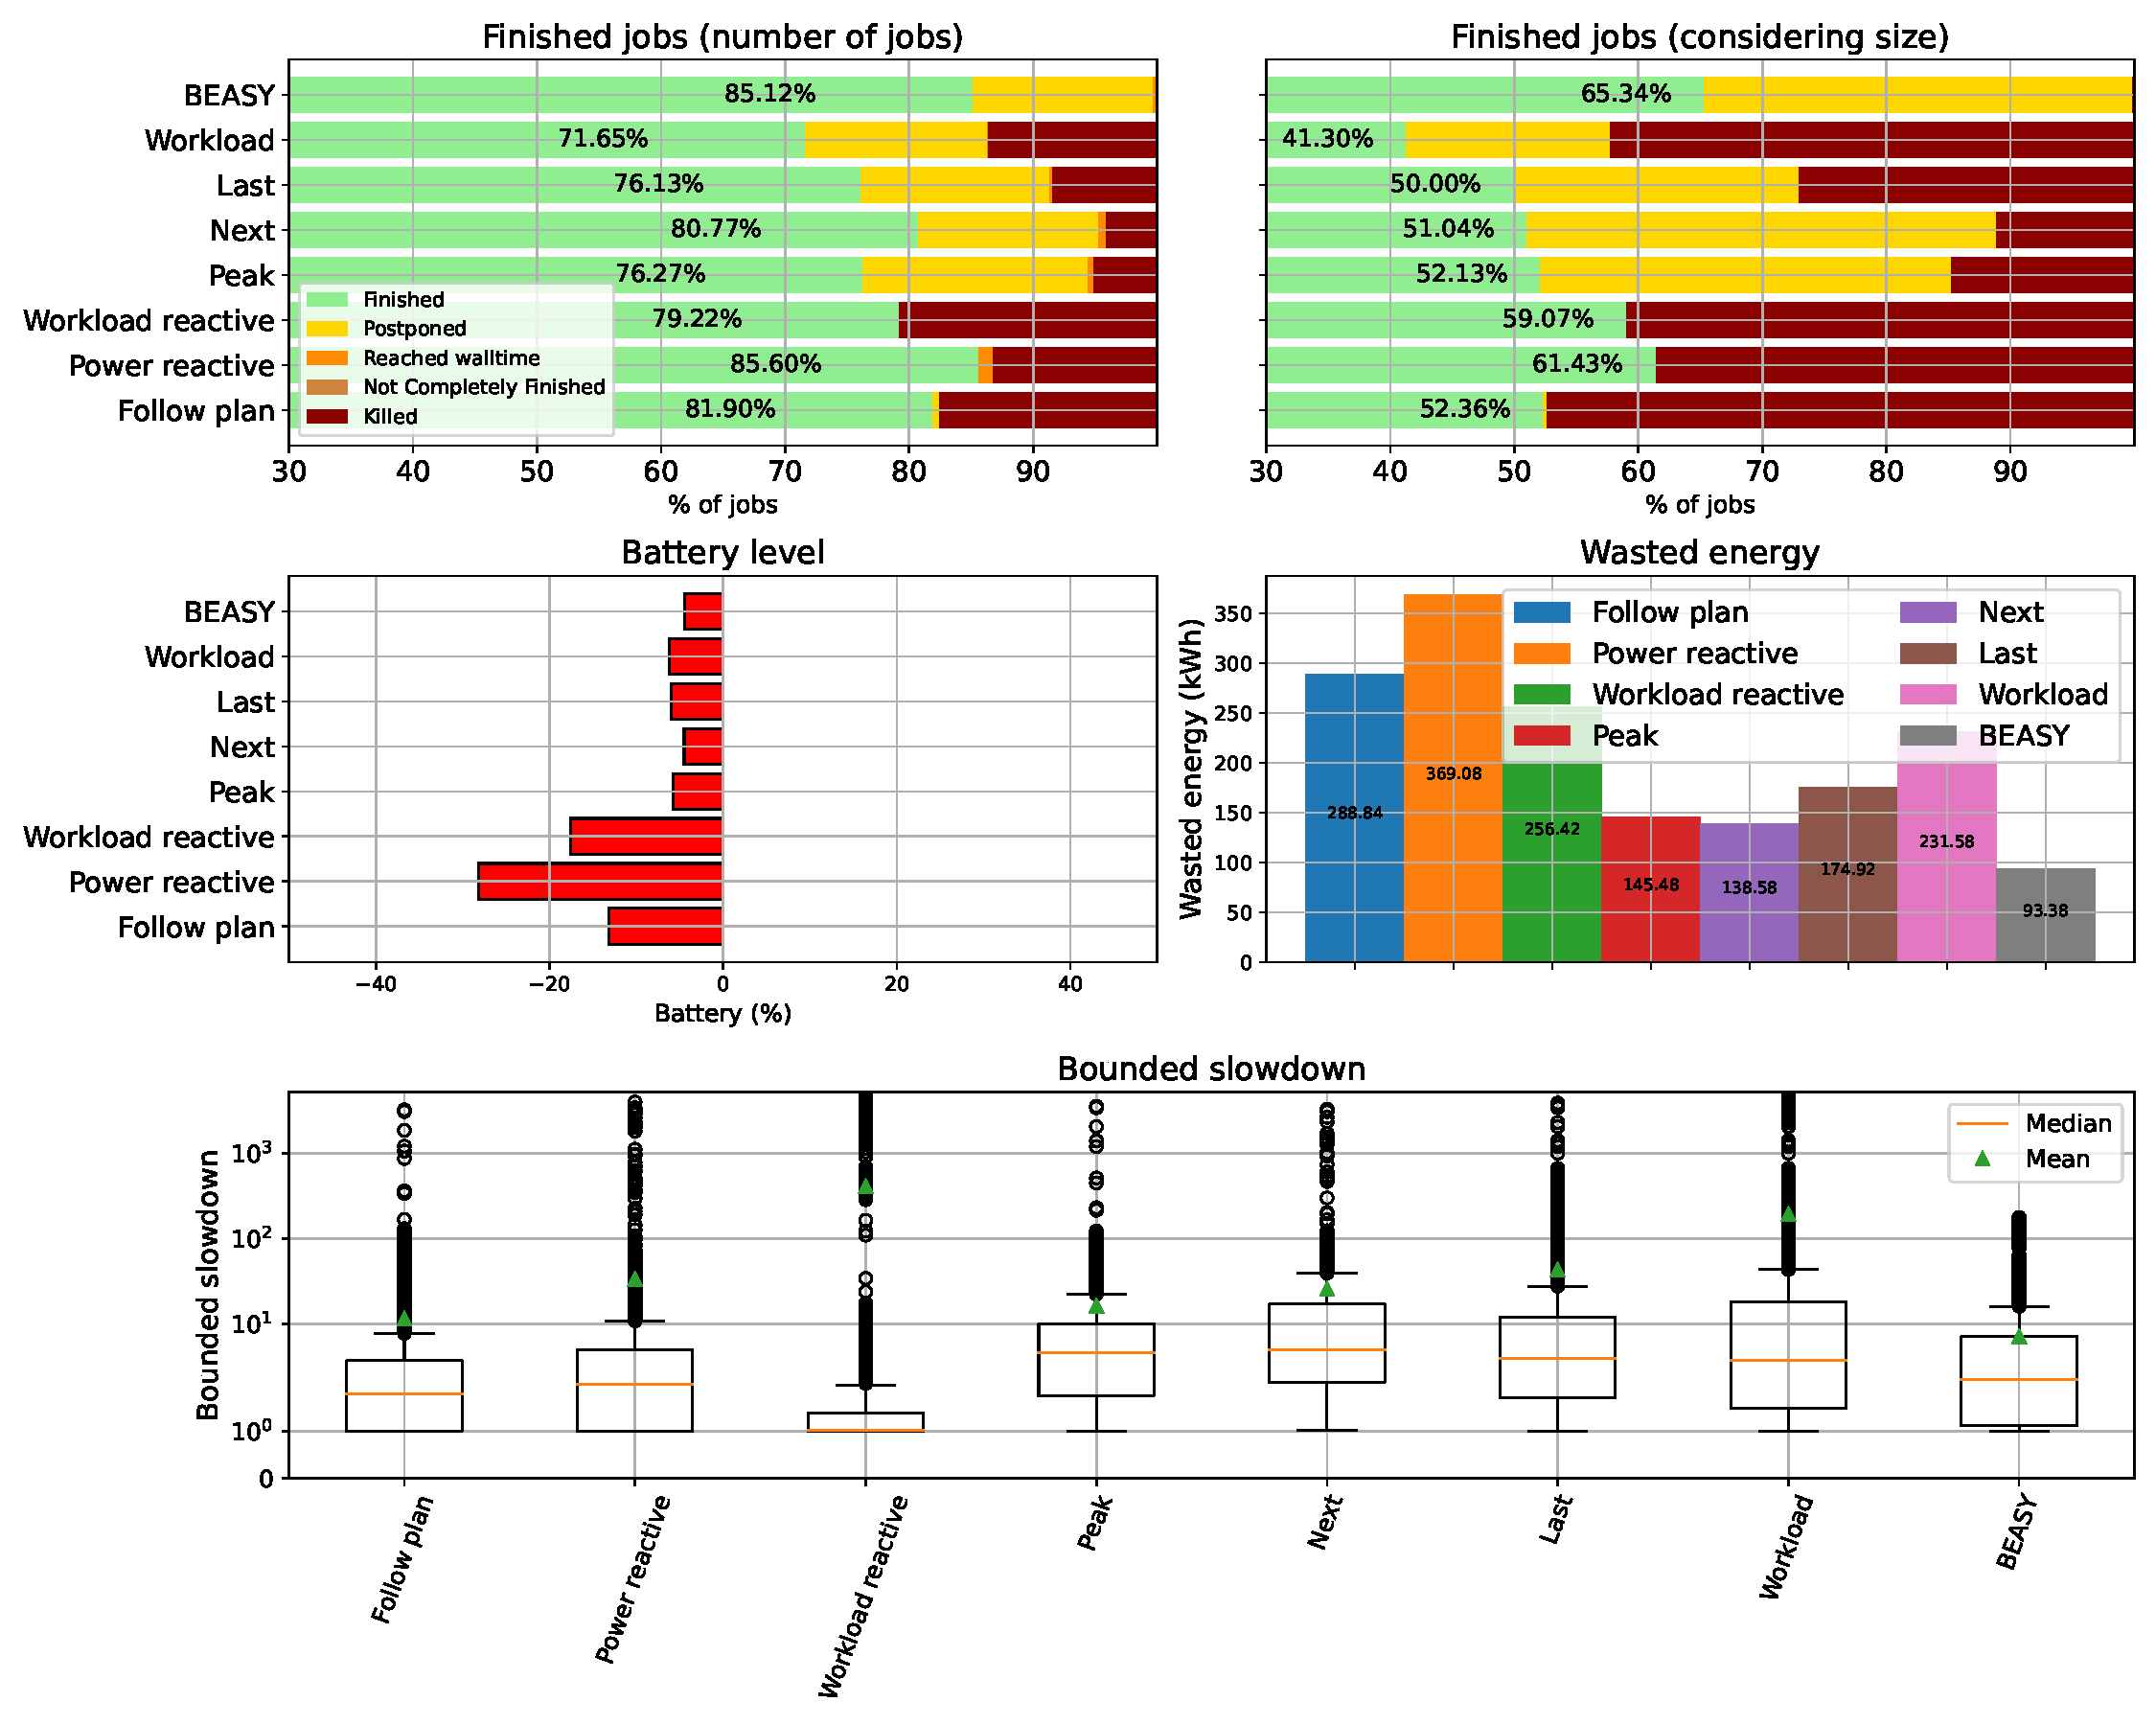
\includegraphics[scale=0.39]{Images/Heuristic/profile_worst_workload_1_with_noise.pdf}
    \caption{Results of \emph{\systemName} on critical case 3.}
    \label{fig:beasy_critical_3}
\end{figure}

\clearpage

\subsubsection{Scenario Critical 4}

The last case is with the profile worst-case and the jobs arriving at the end of the time window. Figure \ref{fig:beasy_critical_4} shows the results. Among the executions that respected the battery level, \emph{\systemName} has the higher finished jobs and lower killed jobs (in number and sizing). All the baselines have more finished jobs than \emph{\systemName} in size. In number, \emph{\systemName} is best than the policies and the \emph{Power reactive}, but finishes less than \emph{Workload reactive} and \emph{Follow plan}. However, \emph{\systemName} kills fewer jobs than all other algorithms. We can see that \emph{Workload reactive} finishes in number almost the same percentage as \emph{\systemName} but finishes far from the battery target level. This scenario is hard to start big jobs, resulting in a big impact on the size of the jobs executed by \emph{\systemName}. Again, \emph{\systemName} has an outstanding result regarding wasted energy. It wastes less energy than all the other algorithms, with 19.70\% less than the second-best, \emph{Workload policy}. Finally, in this case, \emph{\systemName} has a higher median bounded slowdown compared to the other algorithms, but the \emph{Next} policy. The mean value of \emph{\systemName} is similar to \emph{Workload}, \emph{Last}, and \emph{Power reactive} but higher than \emph{Follow plan} and \emph{Workload reactive}. \emph{\systemName} finishes more small jobs due to the power constraints, in which the waiting time has higher importance. Since our bounded slowdown considers only the finished jobs, executing more small jobs can produce a higher slowdown.

\begin{figure}[!htb]
    \centering
    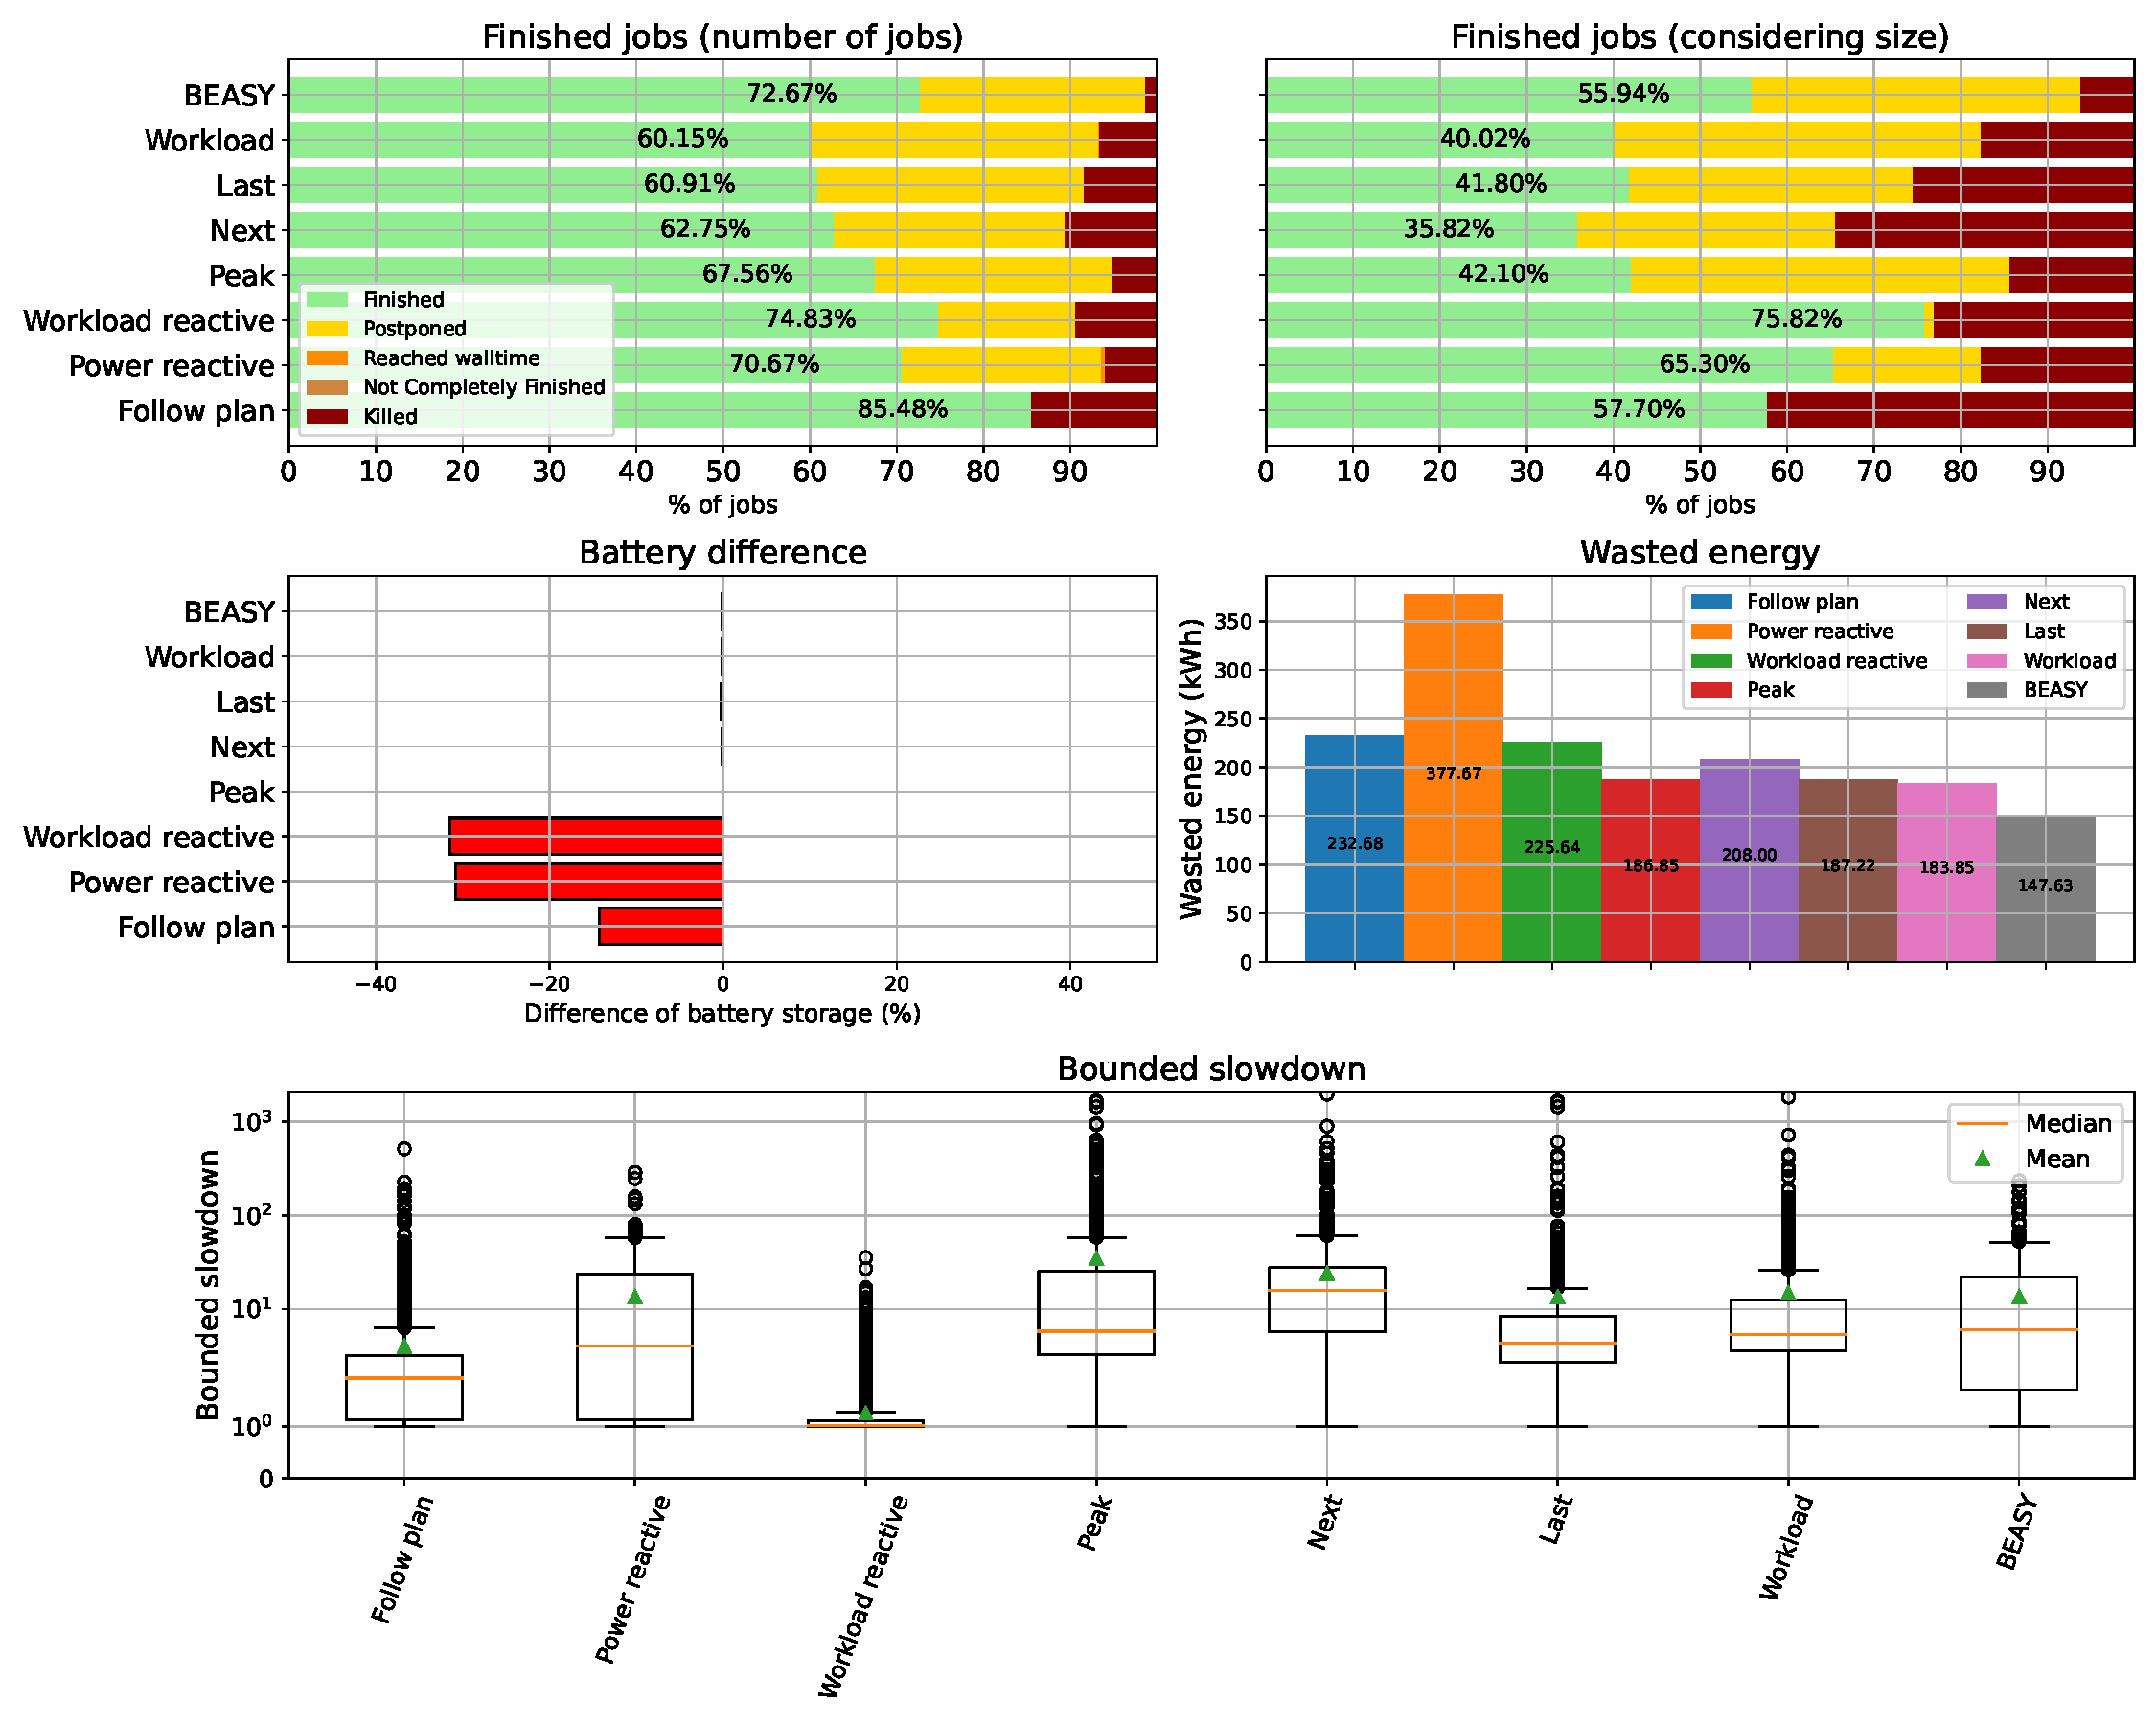
\includegraphics[scale=0.39]{Images/Heuristic/profile_worst_workload_2_with_noise.pdf}
    \caption{Results of \emph{\systemName} on critical case 4.}
    \label{fig:beasy_critical_4}
\end{figure}

\clearpage

\subsection{Average cases}

After presenting the critical cases, this section details the average cases. As mentioned previously, we have taken ten different profiles and workloads. Figure \ref{fig:beasy_average} illustrates the results of the ten executions. Like in the critical cases, \emph{\systemName} presents the lowest number of killed jobs. \emph{\systemName} has no execution with more than 5\% (in number) or 20\% (in size) of killed jobs. The other algorithms have a higher mean and worst-case. For example, \emph{Workload reactive} has two executions with more than 20\% killed jobs in number and one execution with more than 50\% in size. The policies reduce these numbers but have higher values than \emph{\systemName}. Considering finished jobs, \emph{\systemName} has the second-best mean of 93.29\% (in number) and 85.42 (in size). \emph{Workload reactive} Workload reactive has the best mean with 97.27\% (in number) and 90.86 (in size). \emph{Workload reactive} is very aggressive, which helps to have a higher number of finished jobs but also leads to a high killed job number. Figure \ref{fig:soc_average} compares the state of charge of \emph{Workload reactive} and \emph{\systemName} in the execution where \emph{Workload reactive} killed several jobs. \emph{Workload reactive} could not avoid the 20\% threshold, resulting in several killed jobs. \emph{\systemName} avoids this threshold.

\begin{figure}[!htb]
    \centering
    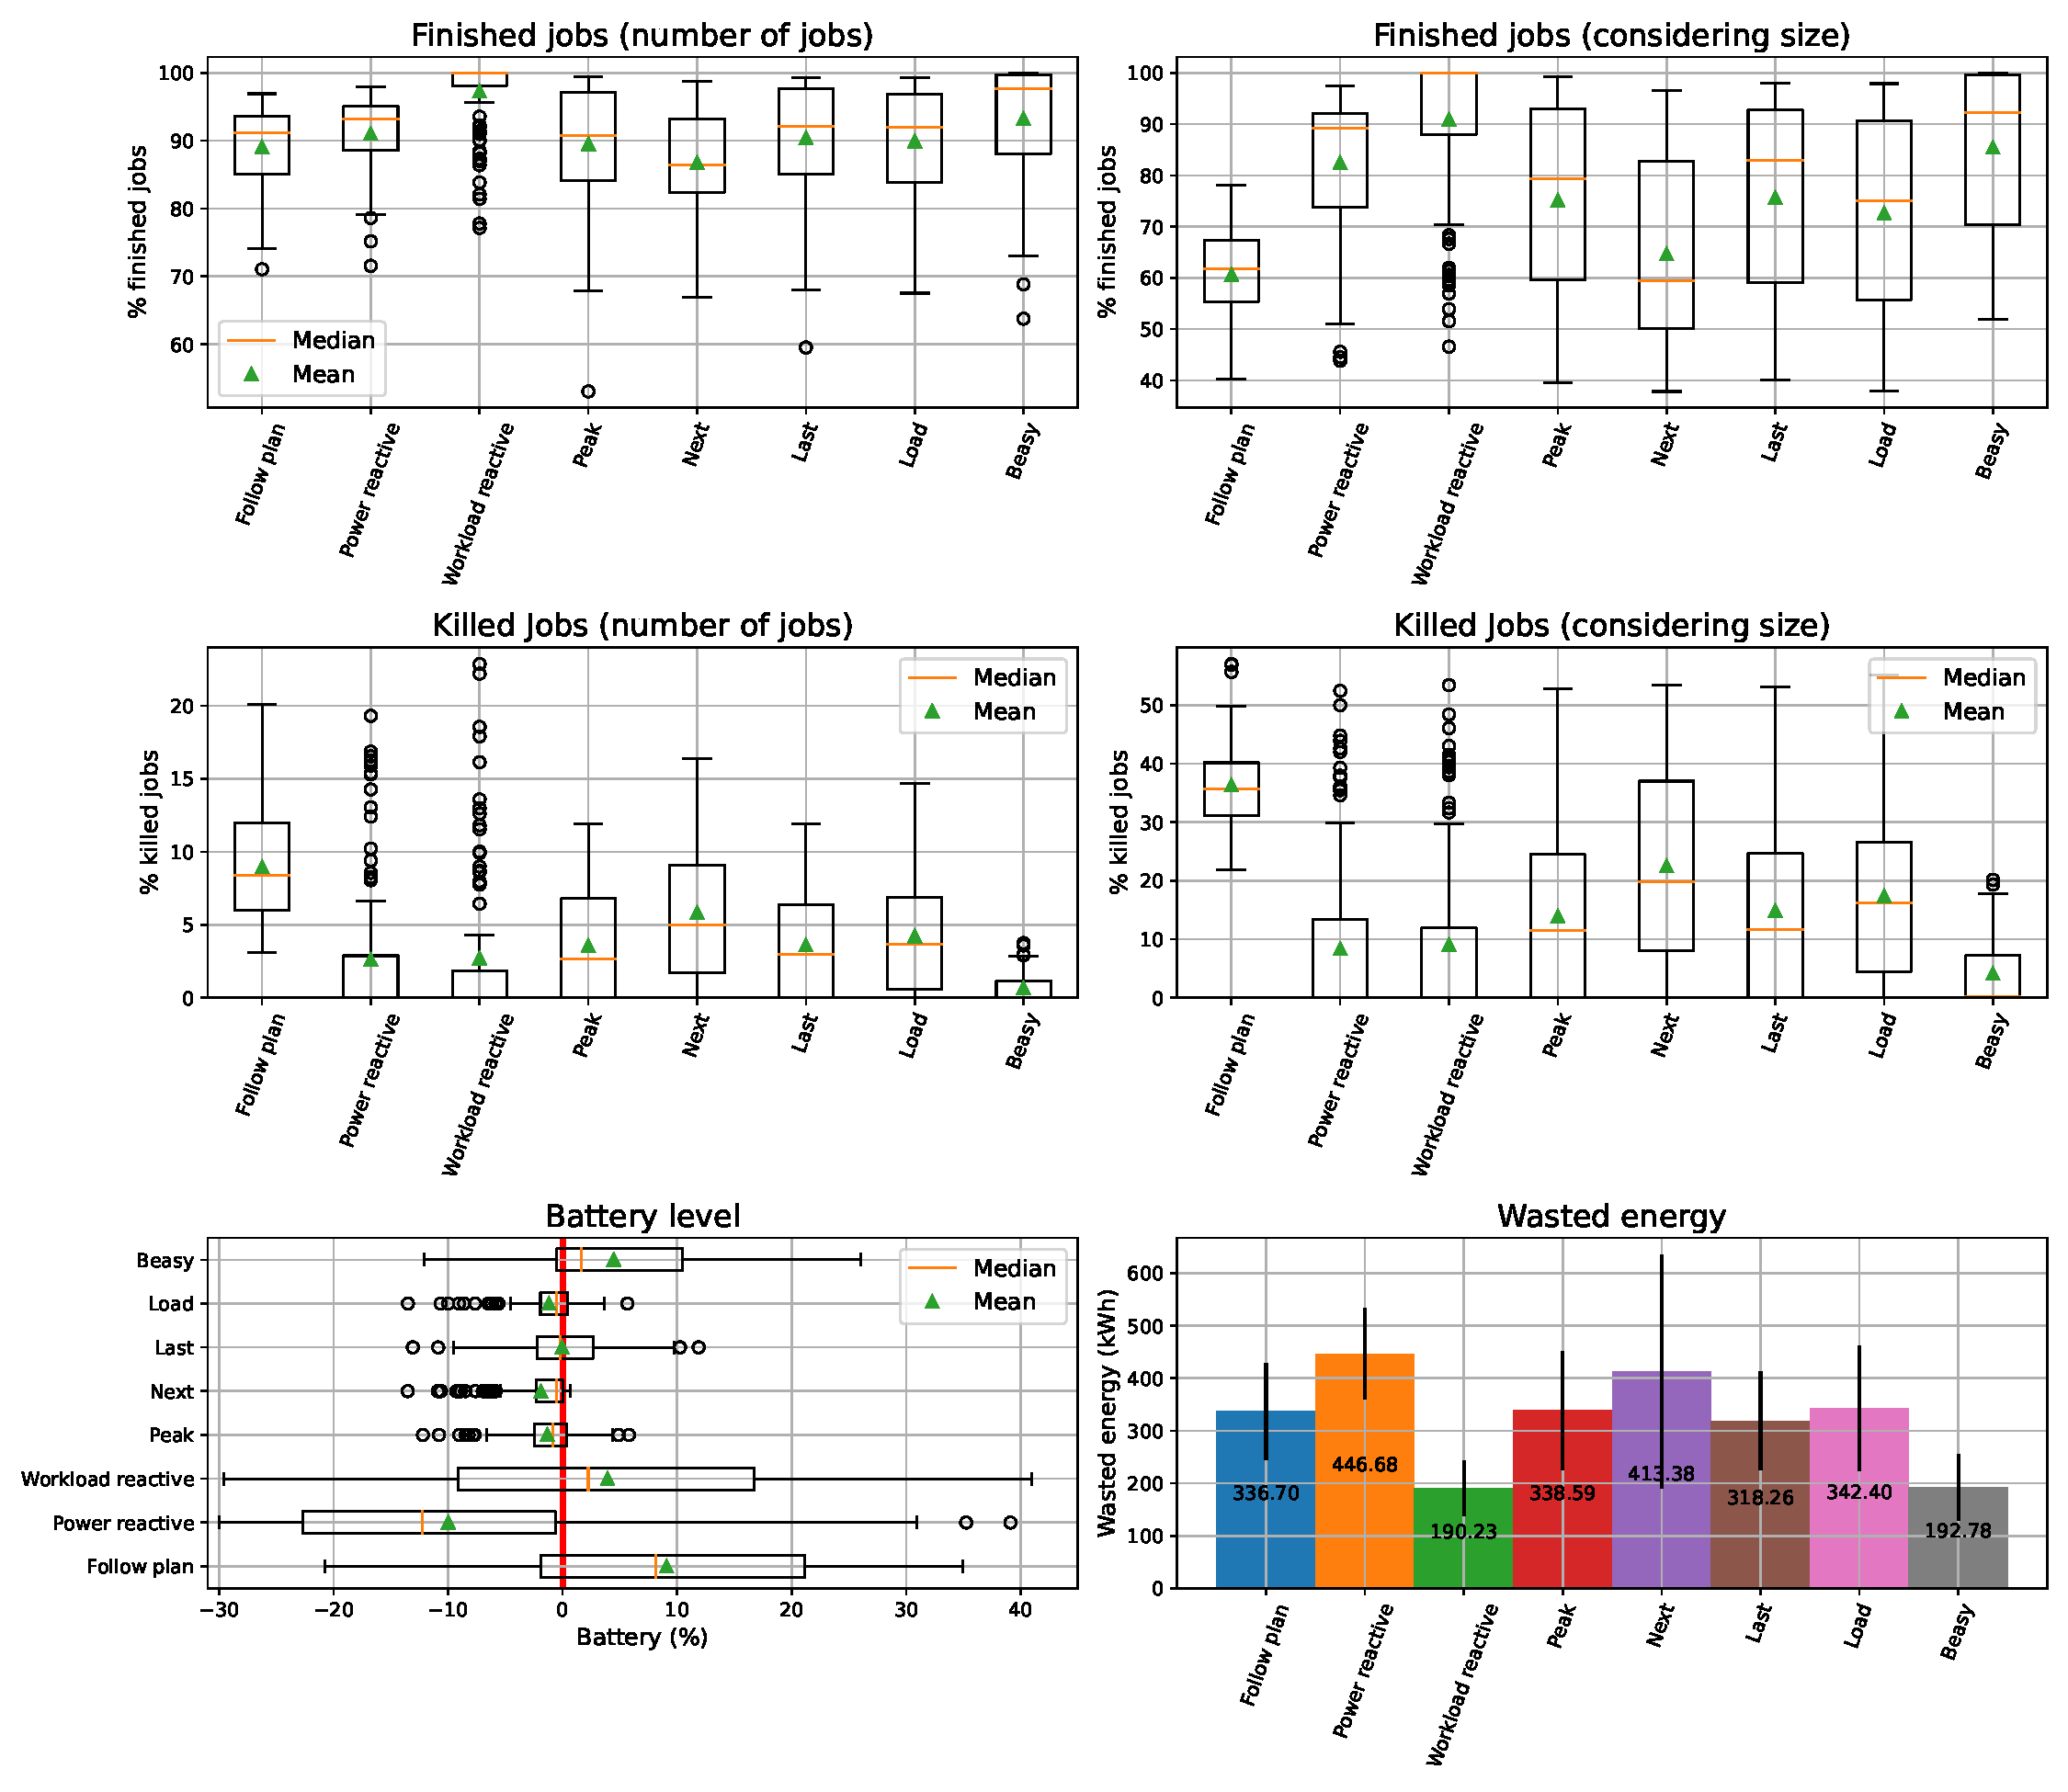
\includegraphics[scale=0.39]{Images/Heuristic/100_cases.pdf}
    \caption{Results of \emph{\systemName} on average cases.}
    \label{fig:beasy_average}
\end{figure}

\begin{figure}[!htb]
    \centering
    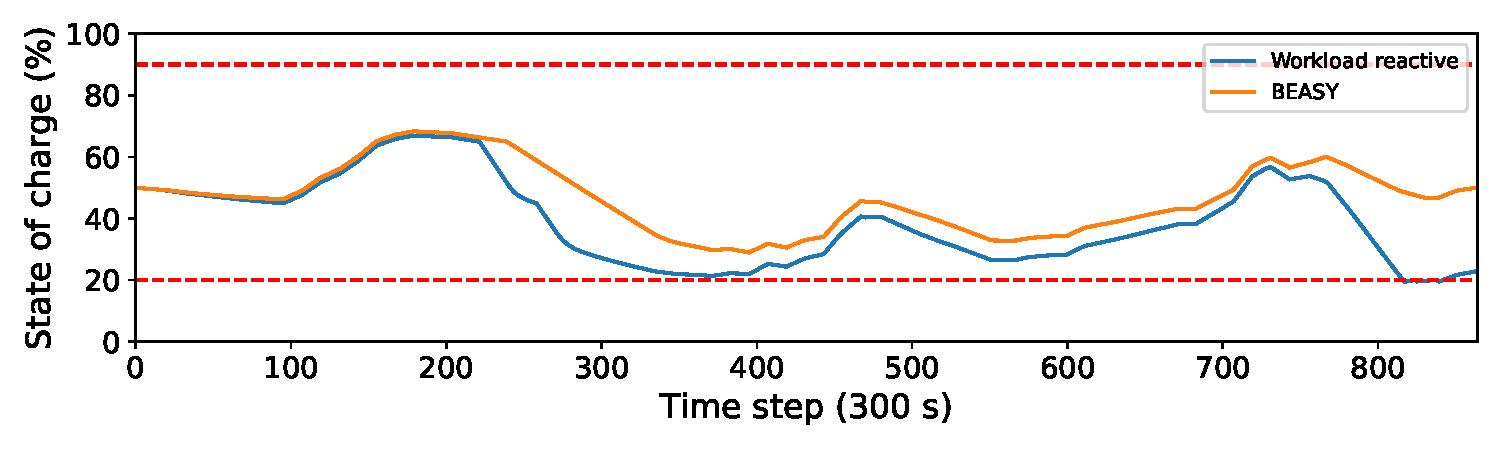
\includegraphics[scale=0.5]{Images/Heuristic/diff_state_of_charge.pdf}
    \caption{State of charge in one of the scenarios. \emph{Workload reactive} kills several jobs when the battery is lower than 20\%. \emph{\systemName} avoids this threshold and could maintain the jobs running.}
    \label{fig:soc_average}
\end{figure}

Comparing the number of jobs killed, \emph{Workload reactive} has 19\% of the executions above 5\% of killed jobs (in number), while \emph{\systemName} has none. This result shows that \emph{\systemName} can maintain the state of charge in control. Also, \emph{Workload reactive} has the two worst number of jobs killed among all executions. \emph{Power reactive} has the third-best number of completed jobs but also 19\% of the executions above 5\% of killed jobs (in number). Considering the battery target level, \emph{\systemName} has good levels since it is near the target level (average of 54.47\%). 75\% of the executions in \emph{\systemName} finished with the battery at the target level or higher. While \emph{Workload reactive} has a wider battery level, with the minimal being close to -30\%, \emph{\systemName} has a better result. The best executions in this metric are the policies (\emph{Peak}, \emph{Next}, \emph{Last}, and \emph{Workload}), always around 50\% and with a very low standard deviation. But, we could see they can not reduce the killed jobs as much as \emph{\systemName}. Finally, \emph{\systemName} and \emph{Workload reactive} have the best result in wasted energy, well below the other executions. \emph{Workload reactive} is very energy aware since it tends to maintain running only the servers needed due to its DPM technique. So, being close to the same result is quite outstanding for \emph{\systemName}. 

\subsection{Discussion}

After presenting the results of critical and average cases, this section consolidates our discussion. Table \ref{tab:ranking} ranks all algorithm results over the different tested scenarios. We highlight in green the top-3 results on each metric for each scenario. The bottom-3 results are in red. Both finished and killed jobs are considered in number. Killed jobs are: killed jobs + reach the walltime + not completely finished. For SoC, we assume the best results as the higher real SoC at the end of the time window. This table highlights the excellent results of \emph{\systemName} over the different experiments, where it finishes in top-3 in all cases. \emph{\systemName} is always the best one in killed jobs. This heuristic can identify when it is possible to execute more jobs and when it is better to be conservative, postponing some jobs. Running everything is not always possible due to power constraints in our data center environment. Postponing the jobs allows us to plan the next time window considering them. For example, the next time window could use more energy coming from hydrogen to deal with these jobs. In an online way, it is not possible to change the hydrogen usage since it has a warm-up time. Also, offline can consider the seasonality of renewable production in its decision (e.g., spend more energy from hydrogen in winter and recharge it in summer). Even postponing jobs, \emph{\systemName} is always between the top 3 finished jobs. 

The worst result of \emph{\systemName} is third place in finished jobs in critical case 4 (Profile worst-case and workload in the end). This critical case is complicated to guarantee the execution of all jobs. The algorithm with the highest finished jobs metric (\emph{Follow plan}) also has the highest killed jobs in this scenario Also, the second-best (\emph{Workload reactive}) is the third-worst in killed jobs. On the other hand, \emph{\systemName} is the third-best in finished jobs and the best in killed jobs. \emph{Follow plan} and \emph{Workload reactive} also have worse SoC level than \emph{\systemName}. Regarding the average cases, \emph{Workload reactive} seems a good possibility. However, the third place in SoC (considering the mean) does not illustrate the variance in the state of charge. Figure \ref{fig:beasy_average} shows that this algorithm varies its SoC, being very unstable. \emph{\systemName} has the second-best SoC. We can see in Figure \ref{fig:beasy_average} that \emph{\systemName} has a higher SoC variance than the policies, but it is still lower than the baselines. Also, 75\% of its values are higher than the target level, showing that it usually finishes with more energy to use in the next time window. \emph{Follow plan} has a similar result in SoC, but this algorithm has the worst killed jobs and second-worst finished jobs. \emph{Follow plan} saves battery because it does not adapt its plan to improve QoS (finished/killed jobs). 

Besides, \emph{\systemName} also has good wasted energy over all executions. It has the best wasted energy three times and the second-best two times. The only algorithm with better results is \emph{Workload reactive}. We expected \emph{Workload reactive} to have good wasted energy since it reacts to job arrival and applies DPM to turn off the servers. Even so, \emph{\systemName} outperforms \emph{Workload reactive} in three of five scenarios. In the average cases, \emph{Workload reactive} has lower wasted energy than \emph{\systemName}, but with a very similar result. \emph{Workload reactive} has two high wasted energy results in the scenarios with lower power production due to the high number of killed jobs. Besides \emph{\systemName}, only \emph{Last} policy has no wasted energy in the bottom-3. However, it is always in third or fourth place.

Finally, let's compare \emph{\systemName} globally. \emph{\systemName} has the best overall results, showing a balanced algorithm. As mentioned before, it finishes in top-3 in all cases. \emph{Workload reactive} also has several good results, mainly regarding job metrics. However, it is too aggressive, which is not a good approach in critical cases 1 and 3 (with more jobs on the first day). On the other hand, following strictly the plan in a conservative way (\emph{Follow plan}) is not a good approach either. The proposed policies are the first step away from being too conservative, showing some good results. For example, \emph{Last} policy has only two bottom-3 QoS results in the scenarios with less energy. However, they are still not enough. \emph{\systemName} can find a balance between QoS and power constraints. The SoC predictions help the SoC to finish close to the target. The finished and killed jobs have good results in \emph{\systemName} due to its scheduling approach. The \emph{\systemName}'s scheduling validation helps to guarantee job executions. Finally, the wasted energy good results come from both scheduling and SoC predictions. Executing small jobs in dangerous moments maintains the SoC under control and reduces killed jobs. Reducing killed jobs also reduces wasted energy. So, combining good scheduling and power compensation decisions makes \emph{\systemName} achieve these outstanding results.

\begin{landscape}

\begin{table*}[htp]
    \centering
    \caption{Consolidate average results in every scenario.}
    \label{tab:ranking}
    \begin{tabular}{c|l||l|l|l|l|l|l|l|l}
        \hline
        Scenario                                                                                                       & Metric        & Follow plan                   & Power reactive                & Workload reactive             & Peak                          & Next                          & Last                          & Load                      & BEASY                         \\ \hline\hline
        \multirow{4}{*}{\begin{tabular}[c]{@{}c@{}}Profile best-case \\ and \\ workload in \\ beginning\end{tabular}}  & Finished jobs & {\cellcolor{red!75}}\nth{8}   & {\cellcolor{red!50}}\nth{7}   & {\cellcolor{red!25}}\nth{6}   & \nth{4}                       & \nth{5}                       & {\cellcolor{green!50}}\nth{2} & {\cellcolor{green!25}}\nth{3} & {\cellcolor{green!75}}\nth{1} \\ 
        \hhline{~---------}
                                                                                                                       & Killed jobs   & {\cellcolor{red!75}}\nth{8}   & {\cellcolor{red!50}}\nth{7}   & {\cellcolor{red!25}}\nth{6}   & \nth{4}                       & \nth{5}                       & {\cellcolor{green!50}}\nth{2} & {\cellcolor{green!25}}\nth{3} & {\cellcolor{green!75}}\nth{1} \\ \hhline{~---------}
                                                                                                                       & SoC           & {\cellcolor{green!75}}\nth{1} & {\cellcolor{red!75}}\nth{8}   & {\cellcolor{green!25}}\nth{3} & {\cellcolor{red!25}}\nth{6}   & {\cellcolor{red!50}}\nth{7}   & \nth{4}                       & \nth{5}                       & {\cellcolor{green!50}}\nth{2} \\ \hhline{~---------}
                                                                                                                       & Wasted energy & {\cellcolor{red!50}}\nth{7}   & {\cellcolor{red!75}}\nth{8}   & {\cellcolor{green!50}}\nth{2} & \nth{4}                       & {\cellcolor{red!25}}\nth{6}   & {\cellcolor{green!25}}\nth{3} & \nth{5}                       & {\cellcolor{green!75}}\nth{1} \\ \hline\hline
        \multirow{4}{*}{\begin{tabular}[c]{@{}c@{}}Profile best-case \\ and \\ workload in end\end{tabular}}           & Finished jobs & {\cellcolor{red!50}}\nth{7}   & \nth{4}                       & {\cellcolor{green!75}}\nth{1} & {\cellcolor{red!25}}\nth{6}   & {\cellcolor{red!75}}\nth{8}   & {\cellcolor{green!25}}\nth{3} & \nth{5}                       & {\cellcolor{green!50}}\nth{2} \\ \hhline{~---------}
                                                                                                                       & Killed jobs   & {\cellcolor{red!75}}\nth{8}   & \nth{5}                       & {\cellcolor{green!75}}\nth{1} & {\cellcolor{red!25}}\nth{6}   & {\cellcolor{red!50}}\nth{7}   & \nth{4}                       & {\cellcolor{green!25}}\nth{3} & {\cellcolor{green!75}}\nth{1} \\ \hhline{~---------}
                                                                                                                       & SoC           & {\cellcolor{green!75}}\nth{1} & {\cellcolor{red!75}}\nth{8}   & {\cellcolor{red!50}}\nth{7}   & {\cellcolor{green!25}}\nth{3} & \nth{4}                       & \nth{5}                       & {\cellcolor{red!25}}\nth{6}   & {\cellcolor{green!50}}\nth{2} \\ \hhline{~---------}
                                                                                                                       & Wasted energy & \nth{5}                       & {\cellcolor{red!75}}\nth{8}   & {\cellcolor{green!75}}\nth{1} & {\cellcolor{red!25}}\nth{6}   & {\cellcolor{red!50}}\nth{7}   & {\cellcolor{green!25}}\nth{3} & \nth{4}                       & {\cellcolor{green!50}}\nth{2} \\ \hline\hline
        \multirow{4}{*}{\begin{tabular}[c]{@{}c@{}}Profile worst-case \\ and \\ workload in \\ beginning\end{tabular}} & Finished jobs & {\cellcolor{green!25}}\nth{3} & {\cellcolor{green!75}}\nth{1} & \nth{5}                       & {\cellcolor{red!25}}\nth{6}   & \nth{4}                       & {\cellcolor{red!50}}\nth{7}   & {\cellcolor{red!75}}\nth{8}   & {\cellcolor{green!50}}\nth{2} \\ \hhline{~---------}
                                                                                                                       & Killed jobs   & {\cellcolor{red!50}}\nth{7}   & {\cellcolor{red!25}}\nth{6}   & {\cellcolor{red!75}}\nth{8}   & {\cellcolor{green!25}}\nth{3} & {\cellcolor{green!50}}\nth{2} & \nth{4}                       & \nth{5}                       & {\cellcolor{green!75}}\nth{1} \\ \hhline{~---------}
                                                                                                                       & SoC           & {\cellcolor{red!25}}\nth{6}   & {\cellcolor{red!75}}\nth{8}   & {\cellcolor{red!50}}\nth{7}   & {\cellcolor{green!25}}\nth{3} & {\cellcolor{green!50}}\nth{2} & \nth{4}                       & \nth{5}                       & {\cellcolor{green!75}}\nth{1} \\ \hhline{~---------}
                                                                                                                       & Wasted energy & {\cellcolor{red!50}}\nth{7}   & {\cellcolor{red!75}}\nth{8}   & {\cellcolor{red!25}}\nth{6}   & {\cellcolor{green!25}}\nth{3} & {\cellcolor{green!50}}\nth{2} & \nth{4}                       & \nth{5}                       & {\cellcolor{green!75}}\nth{1} \\ \hline\hline
        \multirow{4}{*}{\begin{tabular}[c]{@{}c@{}}Profile worst-case \\ and \\ workload in end\end{tabular}}          & Finished jobs & {\cellcolor{green!75}}\nth{1} & \nth{4}                       & {\cellcolor{green!50}}\nth{2} & \nth{5}                       & {\cellcolor{red!25}}\nth{6}   & {\cellcolor{red!50}}\nth{7}   & {\cellcolor{red!75}}\nth{8}   & {\cellcolor{green!25}}\nth{3} \\ \hhline{~---------}
                                                                                                                       & Killed jobs   & {\cellcolor{red!75}}\nth{8}   & {\cellcolor{green!25}}\nth{3} & {\cellcolor{red!25}}\nth{6}   & {\cellcolor{green!50}}\nth{2} & {\cellcolor{red!50}}\nth{7}   & \nth{5}                       & \nth{4}                       & {\cellcolor{green!75}}\nth{1} \\ \hhline{~---------}
                                                                                                                       & SoC           & {\cellcolor{red!25}}\nth{6}   & {\cellcolor{red!50}}\nth{7}   & {\cellcolor{red!75}}\nth{8}   & {\cellcolor{green!75}}\nth{1} & {\cellcolor{green!25}}\nth{3} & \nth{5}                       & \nth{4}                       & {\cellcolor{green!50}}\nth{2} \\ \hhline{~---------}
                                                                                                                       & Wasted energy & {\cellcolor{red!50}}\nth{7}   & {\cellcolor{red!75}}\nth{8}   & {\cellcolor{red!25}}\nth{6}   & {\cellcolor{green!25}}\nth{3} & \nth{5}                       & \nth{4}                       & {\cellcolor{green!50}}\nth{2} & {\cellcolor{green!75}}\nth{1} \\ \hline\hline
        \multirow{4}{*}{100 average cases}                                                                             & Finished jobs & {\cellcolor{red!50}}\nth{7}   & {\cellcolor{green!25}}\nth{3} & {\cellcolor{green!75}}\nth{1} & {\cellcolor{red!25}}\nth{6}   & {\cellcolor{red!75}}\nth{8}   & \nth{4}                       & \nth{5}                       & {\cellcolor{green!50}}\nth{2} \\ \hhline{~---------}
                                                                                                                       & Killed jobs   & {\cellcolor{red!75}}\nth{8}   & {\cellcolor{red!25}}\nth{6}   & {\cellcolor{green!50}}\nth{2} & \nth{4}                       & {\cellcolor{red!50}}\nth{7}   & {\cellcolor{green!25}}\nth{3} & \nth{5}                       & {\cellcolor{green!75}}\nth{1} \\ \hhline{~---------}
                                                                                                                       & SoC           & {\cellcolor{green!75}}\nth{1} & {\cellcolor{red!75}}\nth{8}   & {\cellcolor{green!25}}\nth{3} & {\cellcolor{red!25}}\nth{6}   & {\cellcolor{red!50}}\nth{7}   & \nth{4}                       & \nth{5}                       & {\cellcolor{green!50}}\nth{2} \\ \hhline{~---------}
                                                                                                                       & Wasted energy & \nth{4}                       & {\cellcolor{red!75}}\nth{8}   & {\cellcolor{green!75}}\nth{1} & \nth{5}                       & {\cellcolor{red!50}}\nth{7}   & {\cellcolor{green!25}}\nth{3} & {\cellcolor{red!25}}\nth{6}   & {\cellcolor{green!50}}\nth{2} \\ \hline
    \end{tabular}
\end{table*}

\end{landscape}

\section{Conclusion}

This chapter presented and evaluated \emph{\systemName}, a heuristic that mixes power and scheduling decisions. \emph{\systemName} uses power production and demand predictions to estimate the state of charge. This SoC estimation helps to make better power compensation decisions. Also, \emph{\systemName} identifies dangerous moments where the SoC could be too close to the battery's lower boundary. In these dangerous moments, \emph{\systemName} starts to be conservative, preferring to run small over big jobs. On the scheduling side, it validates if the job can run entirely. It verifies if the job's servers are available during the entire execution or if it is possible to migrate energy to maintain the servers running. We compared \emph{\systemName} with three baselines (\emph{Follow plan}, \emph{Power reactive}, and \emph{Workload reactive}) and the four policies presented in Chapter \ref{cha:power_compensations}. \emph{\systemName} showed outstanding results in finished jobs, killed jobs, SoC difference from the target, and wasted energy. It is in the top-3 of all metrics in every scenario. 